\section{Belzel}

\textbf{Name}: Belzel \\
\textbf{Function}: Helper

\subsection{Internal World}

\textbf{Age \& Gender}: 347, Male \\
\textbf{Values \& Virtues}: Man of his word  \\
\textbf{Personality}: Quiet, loner, helpful, kind \\
\textbf{Interests}: Meditation, inner peace \\
\textbf{Ethnic Group}: Arabic Djinn

\subsection{External World}
\textbf{Environment}: Desert in the South of Ingary.  \\
\textbf{Education}: High-educated. \\
\textbf{Social \& Cultural Background}: He has left society many decades ago and he is used to live alone. \\
\textbf{Look \& Feel}: He looks like a 50-years-old fat man with long beard. \\
\textbf{Job \& Experience}: He is a powerful wizard. \\
\\
\textbf{Relatives \& Relation}:
\begin{enumerate}
\item \textbf{Sophie and Calcifer}: He  is glad to help them because he feels they really need his help.
\item \textbf{Howl, Justine, Mizar}: No one knows each other
\item \textbf{Suliman}: He doesn’t know her
\end{enumerate}

\begin{figure}
  \centering
  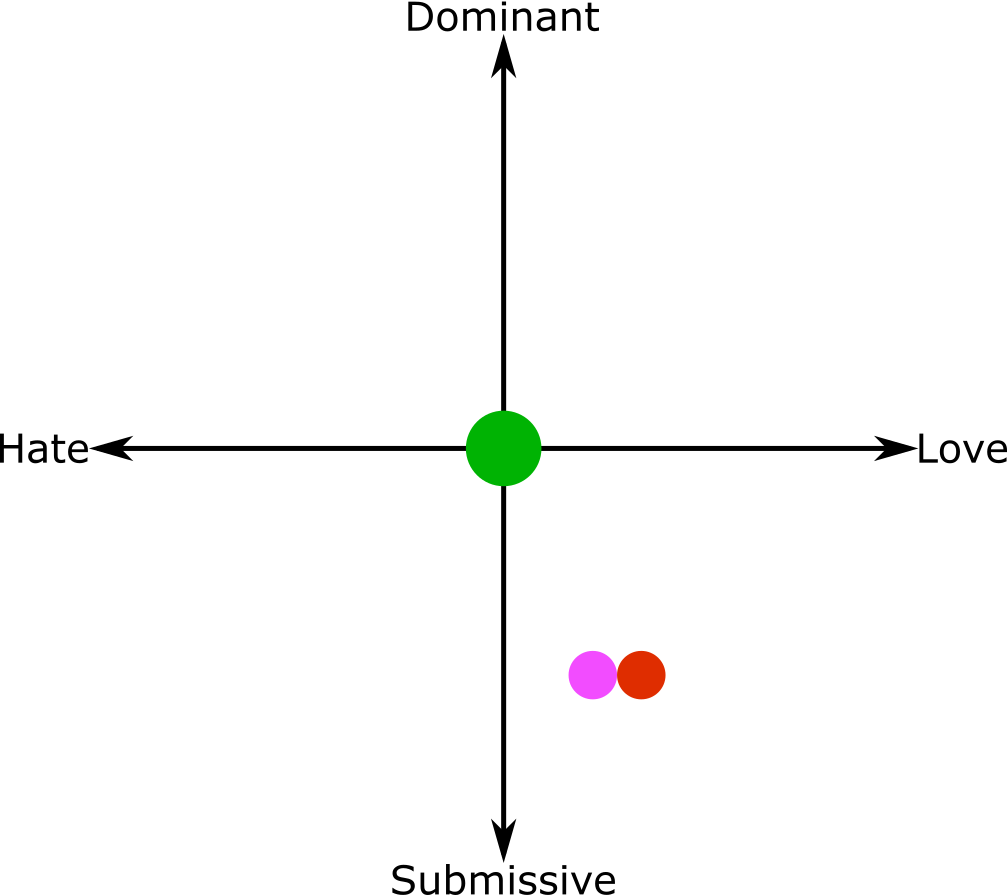
\includegraphics[width=8cm]{Images/Circumplexes/belzelCircumplex}
  \caption{Circumplex of Belzel}
\end{figure}

\begin{figure}
   \centering
    
\includegraphics[width=8cm]{Images/Evolutions/belzelEvolution}
   \caption{Evolutions of Belzel}
\end{figure}

\subsection{Description}
He is a djinn who spends his days meditating and practicing with new spells, he loves being helpful for people who actually need his help. 


\subsection{Background story}
He decided to move centuries ago into the desert because he felt like the society he was living in was too selfish and asked him for help only for futile things 
Nowadays, no one knows him personally but people in the southern kingdom think, according to a common legend that survived across the centuries, he still lives alone in the desert and he can help you when you are really in trouble.



